\documentclass[handout]{beamer}
\usepackage[utf8]{inputenc}
\usepackage{verbatim}

\usetheme{metropolis}
\title{Algorithmique Avancée}
\subtitle{Implémentation}
\author{Julien Roland}

\let\emph\relax % there's no \RedeclareTextFontCommand
\DeclareTextFontCommand{\emph}{\bfseries\em}

\newcommand{\Op}[2]{\texttt{\underline{#1}#2}}
\usepackage{listingsutf8}

\begin{document}
\lstset{language=c++, basicstyle=\small, columns=fullflexible, inputencoding=utf8/latin1}
\setbeamercovered{dynamic}
\maketitle

\section{C++ : Rappels}

\begin{frame}[t]{Références}
    \begin{itemize}
        \item \href{http://www.informit.com/store/tour-of-c-plus-plus-9780133549010}{\textbf{A Tour of C++}, Bjarne Stroustrup, C++ In Depth, Addison-Wesley, 2013.}
        \item \href{http://www.stroustrup.com/Programming/}{\textbf{Programming : Principles and Practice Using C++}, Bjarne Stroustrup, Addison-Wesley, 2014.}
        \item \href{http://www.stroustrup.com/Programming/lecture-slides.html}{\textbf{Programming - Lecture slides}, Bjarne Stroustrup, 2015.}
        \item \textbf{Professional C++}, Marc Gregoire, Wrox, 3e édition, 2014.
        \item \href{http://isocpp.github.io/CppCoreGuidelines/CppCoreGuidelines}{\textbf{C++ Core Guidelines}}
    \end{itemize}
\end{frame}

\begin{frame}[t]{Compilation en C++14}
    \textbf{GCC: le compilateur C et C++ du projet GNU:}
    \begin{itemize}
        \item \lstinline{g++ -std=c++14 hello.cpp -o hello}
    \end{itemize}
    \textbf{CMake: générateur de projets (Makefile, Visual Studio,...)}
    \begin{itemize}
        \item \lstinline{set(CMAKE_CXX_STANDARD 14)}
    \end{itemize}
    \textbf{qmake: le générateur du projet Qt}
    \begin{itemize}
        \item \lstinline{CONFIG += c++14}
    \end{itemize}
\end{frame}

\begin{frame}[fragile]{Fonctions}
    \lstinputlisting{listings/fonctions.cpp}
\end{frame}

\begin{frame}[fragile]{Fonctions Templates}
    \lstinputlisting{listings/fonctions_templates.cpp}
\end{frame}

\begin{frame}[fragile]{Fonctions Templates : Ambiguïté}
    \lstinputlisting{listings/fonctions_templates_ambigu.cpp}
\end{frame}

\begin{frame}[fragile]{Fonctions Templates : Résolution de l'ambiguïté}
    \lstinputlisting{listings/fonctions_templates_ambigu_resolution.cpp}
\end{frame}

\begin{frame}[fragile]{Classes}
    Une classe est un \emph{type} défini par l'utilisateur
    \lstinputlisting{listings/classe.cpp}
\end{frame}

\begin{frame}[fragile]{Structures et Classes}
    \begin{itemize}
        \item Une structure est une classe dont tous les membres sont \emph{publics} par défaut:
              \begin{lstlisting}
                struct X {
                    int m;
                };
              \end{lstlisting}
        \item Est équivalent à :
              \begin{lstlisting}
                class X {
                public:
                    int m;
                };
              \end{lstlisting}
    \end{itemize}
\end{frame}

\begin{frame}[fragile]{Structure Date}
    \lstinputlisting{listings/struct_date.cpp}
\end{frame}

\begin{frame}[fragile]{Initialisation avec et sans constructeur}
    \lstinputlisting{listings/init.cpp}
\end{frame}

\begin{frame}[fragile]{Initialisation Uniforme}
    \lstinputlisting{listings/uniform_init.cpp}
\end{frame}

\begin{frame}[fragile]{Structure Date avec constructeur} 
    \lstinputlisting{listings/struct_date_constructor.cpp}
\end{frame}

\begin{frame}[fragile]{Structure Date avec constructeur et préconditions}
    \lstinputlisting{listings/struct_date_constructor_precond.cpp}
\end{frame}

\begin{frame}[fragile]{Classe Date}
    L'implémentation d'une classe Date (voir date.h, date.cpp) permet de maintenir l'ensemble des \emph{invariants} afin qu'un objet de type Date soit toujours maintenu dans un état cohérent.
    \lstinputlisting{listings/class_date_squelette.cpp}
\end{frame}

\begin{frame}[fragile]{La classe Vector}
    \lstinputlisting{listings/vector.hpp}
    (voir vector.hpp et vector.cpp)
\end{frame}

\begin{frame}[fragile]{Template: Une classe Vector générique}
    \lstinputlisting{listings/vector_generique.hpp}
\end{frame}

\begin{frame}[fragile]{Template: Une classe Vector générique}
    \lstinputlisting{listings/vector_generique_main.cpp}
\end{frame}

\begin{frame}[fragile]{Template: Une classe Vector générique}
    \lstinputlisting{listings/vector_generique_main_value_type.cpp}
\end{frame}

\section{La librairie de conteneurs}

\begin{frame}[fragile]{Conteneurs}
    \begin{itemize}
        \item Séquentiels : \lstinline{array, vector, dequeue, forward_list, list}
        \item Associatifs : \lstinline{set, map, multiset, multimap}
        \item Associatifs non ordonnés : \lstinline{unordered_set, unordered_map,...}
        \item Adaptateurs : \lstinline{stack, queue, priority_queue}
    \end{itemize}
    \begin{lstlisting}
template<typename T>
std::ostream& operator<<(std::ostream& s, const std::vector<T>& v);

int main() {
    std::vector<std::string> words {"one", "two", "three", "four", "five"};
    std::cout << "words: " << words << '\n';
}
    \end{lstlisting}
\end{frame}

\begin{frame}{La STL}
    \begin{itemize}
        \item STL : Standard Template Library
        \item Librairie conçue par Alex Stepanov (vers 1992, HP labs)
    \end{itemize}
    Séparation des ``préoccupations'' à l'aide du concept d'\emph{itérateur}:
    \begin{itemize}
        \item Les \emph{algorithmes} manipulent des données sans connaissance du conteneur.
        \item Les \emph{conteneurs} stockent des données mais n'ont pas connaissance des algorithmes.
        \item Les interactions entre conteneurs et algorithmes s'effectuent par l'intermédiaire d'\emph{itérateurs}.
    \end{itemize}
\end{frame}

\begin{frame}{Itérateurs}
    Une paire d'itérateurs ``begin'' et ``end'' définit une séquence d'éléments :
    \begin{center}
        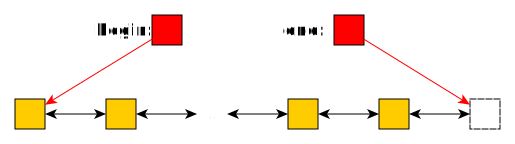
\includegraphics[scale=0.4]{figures/iterateurs.pdf}
    \end{center}
    Un itérateur supporte les opérations suivantes :
    \begin{itemize}
        \item \lstinline{++} : déplacement au prochain élément
        \item \lstinline{*} : accès à l'élément
        \item \lstinline{==} : teste si deux itérateurs réfèrent au même élément
    \end{itemize}
    Certains itérateurs supportent les opérateurs : \lstinline{--, +, -, [], <}.
    Voir \url{http://en.cppreference.com/w/cpp/concept} pour davantage de détails sur les
    différents types d'itérateurs.
\end{frame}

\begin{frame}{Conteneurs}
    \begin{center}
        \emph{std::vector}\\
        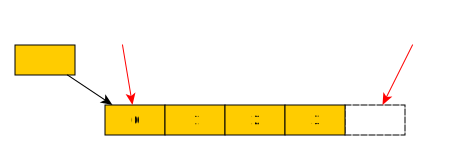
\includegraphics[scale=0.5]{figures/vector.pdf}\\
        \vfill
        \emph{std::list}\\(implémentation traditionnelle: liste doublement chaînée)\\
        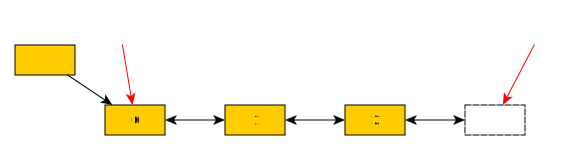
\includegraphics[scale=0.5]{figures/list.pdf}
    \end{center}
\end{frame}

\begin{frame}{Conteneurs}
    \begin{center}
        \emph{std::set}\\(implémentation traditionnelle: arbre rouge-noir)\\
        \vfill
        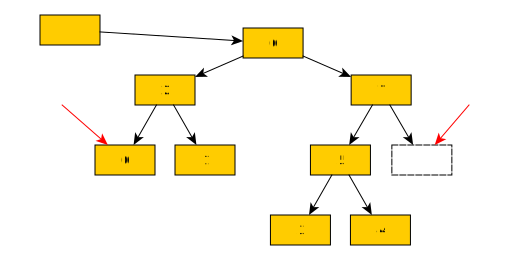
\includegraphics[scale=0.6]{figures/set.pdf}
    \end{center}
\end{frame}

\begin{frame}[fragile]{Conteneurs : std::list et std::vector}
    \lstinputlisting{listings/vector_list_mean.cpp}
\end{frame}

\begin{frame}[fragile]{Conteneurs}
    \emph{Exercice --} Implémenter les fonctions suivantes :
    \begin{lstlisting}
    #include <cmath> // pow
    #include <numeric> // accumulate(InputIt, InputIt, T, BinaryOperation);

    template<typename T>
    T multiplies(T num1, T num2);

    template<typename T>
    T dot(const std::vector<T>& x, const std::vector<T>& y);

    double geometric_mean(const std::vector<double>& x);
    \end{lstlisting}
\end{frame}

\begin{frame}[fragile]{Conteneurs : template}
    \lstinputlisting{listings/containers_mean.cpp}
\end{frame}

\begin{frame}[fragile]{Conteneurs : accès types membres}
    \lstinputlisting{listings/containers_mean_value_type.cpp}
\end{frame}

\begin{frame}[fragile]{Itérateurs}
    \lstinputlisting{listings/containers_mean_iterators.cpp}
\end{frame}

\begin{frame}[fragile]{Conteneurs}
    \emph{Exercice --} Implémenter la fonctions suivants :
    \begin{lstlisting}
    template<typename Iter>
    typename Iter::value_type dot(Iter first1, Iter last1, Iter first2); 
    \end{lstlisting}
\end{frame}


\section{C++ Moderne}

\begin{frame}[t]{Références}
    \begin{itemize}
        \item \href{http://www.informit.com/store/tour-of-c-plus-plus-9780133549010}{A Tour of C++, par Bjarne Stroustrup, C++ In Depth, Addison-Wesley, 2013.}
        \item \href{http://www.stroustrup.com/Programming/}{Programming : Principles and Practice Using C++, par Bjarne Stroustrup, Addison-Wesley, 2014.}
        \item \url{http://en.cppreference.com/w/}
        \item \href{https://herbsutter.com/elements-of-modern-c-style/}{Elements of Modern C++ Style}
        \item \href{http://www.drdobbs.com/cpp/the-c14-standard-what-you-need-to-know/240169034}{The C++14 Standard: What You Need to Know}
        \item \href{http://www.informit.com/articles/article.aspx?p=1852519}{Get to Know the New C++11 Initialization Forms}
    \end{itemize}
\end{frame}

\begin{frame}[fragile]{Auto}
    Au lieu de définir explicitement le type d'une variable, on demande au compilateur de déduire le
    type en utilisant celui de l'expression utilisée pour son initialisation:
    \begin{lstlisting}
    {
        auto x = 1;         // 1 est un entier, alors x est un int
        auto y = 'c';
        auto z = 123'456'789
        auto d = 1.2;
        auto s = "implicite";
        auto s2 = "implicite"s;
        auto sq = sqrt(2);
        auto inconnu;       // erreur
    }
    \end{lstlisting}
\end{frame}

\begin{frame}[fragile]{Boucles basées sur des intervalles}
    \begin{lstlisting}
    std::vector<int> v {31, 1, 464, 233, 12};

    for (int i = 0; i < v.size(); ++i)
        std::cout << v[i] << std::endl;

    for (auto it = v.begin(); it != v.end(); ++it)
        std::cout << *it << std::endl;

    for (int x : v)
        std::cout << x << std::endl;

    for (auto x : v)
        std::cout << x << std::endl;

    for (auto& x : v)
        std::cout << x << std::endl;

    \end{lstlisting}
\end{frame}

\begin{frame}[fragile]{Paramétrer un algorithme à l'aide d'un prédicat}
    Considérons la fonction suivante permettant de compter les occurrences de valeurs dans un
    conteneurs pour lesquelles un prédicat retourne vrai:

    \begin{lstlisting}
template<typename C, typename P>
int count(const C& c, P pred)
{
    int cnt = 0;
    for (const auto& x: c) {
        if (pred(x))
            ++cnt;
    }
    return cnt;
}
    \end{lstlisting}

    Comment utiliser cette fonction afin de déterminer le nombre de valeurs inférieures à une
    constante donnée?
\end{frame}

\begin{frame}[fragile]{Foncteur (objet fonction)}
    \begin{lstlisting}
template<typename C, typename P>
int count(const C& c, P pred);

int main()
{
    std::vector<int> v {31, 1, 464, 233, 12};
    std::cout << count(v, Less_than<int>{42}) << std::endl;
}
    \end{lstlisting}
\end{frame}

\begin{frame}[fragile]{Foncteur (objet fonction)}
    \begin{lstlisting}
template<typename C, typename P>
int count(const C& c, P pred);

template<typename T>
class Less_than {
    const T val;
public:
    Less_than(const T& v): val(v) {}
    bool operator()(const T& x) const { return x < val; }
};

int main()
{
    std::vector<int> v {31, 1, 464, 233, 12};
    std::cout << count(v, Less_than<int>{42}) << std::endl;
}
    \end{lstlisting}
\end{frame}

\begin{frame}[fragile]{Expressions Lambda}
    \begin{lstlisting}
template<typename C, typename P>
int count(const C& c, P pred);

int main()
{
    std::vector<int> v {31, 1, 464, 233, 12};
    std::cout << count(v, [](int x) { return x < 42; }) << std::endl;
}
    \end{lstlisting}

    Une \textit{expression lambda} est une notation permettant de générer implicitement
    un \textit{objet fonction}.
\end{frame}

\begin{frame}[fragile]{Expressions Lambda}
    \begin{lstlisting}
template<typename C, typename P>
int count(const C& c, P pred);

int main()
{
    std::vector<int> v {31, 1, 464, 233, 12};
    int val = 42;
    std::cout << count(v, [&](int x) { return x < val; }) << std::endl;
}
    \end{lstlisting}

    \begin{itemize}
        \item \lstinline{[]} : ne "capture" pas les variables locales
        \item \lstinline{[&]} : indique de \textit{capturer} par référence l'ensemble des variables locales
        \item \lstinline{[=]} : indique de \textit{capturer} par copie l'ensemble des variables locales
        \item Quelques exemples : \lstinline{[=x], [&x], [&x, &v]} 
    \end{itemize}
\end{frame}


\section{Bibliothèque algorithmique}

\begin{frame}[fragile]{Exercices}
    Référence : \url{http://en.cppreference.com/w/cpp/algorithm}\\
    \vfill
    Considérons un ensemble de valeurs entières contenues dans un \lstinline{std::vector<int>}. Utiliser les fonctions de la bibliothèque algorithmique afin de résoudre de manière efficace les problèmes suivants :
    \begin{enumerate}
        \item Déterminer si toutes les valeurs sont positives ou nulles.
        \item Remplacer toutes les valeurs négatives par 0.
        \item Afficher toutes les valeurs positives (utiliser un \lstinline{std::ostream_iterator}).
        \item Déterminer la position du premier et du dernier élément négatif.
    \end{enumerate}
\end{frame}

\begin{frame}[fragile]{Palindrome}
    \begin{lstlisting}
template< class InputIt1, class InputIt2 >
bool equal( InputIt1 first1, InputIt1 last1, InputIt2 first2 );

bool is_palindrome(const std::string& s)
{
    return std::equal(s.begin(), s.begin() + s.size()/2, s.rbegin());
}
    \end{lstlisting}
\end{frame}

\begin{frame}[fragile]{Tri par insertion}
    \begin{center}
        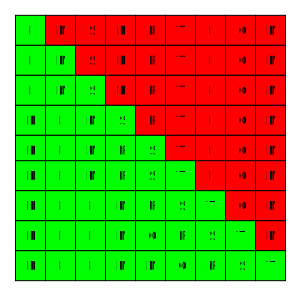
\includegraphics[scale=0.6]{figures/insertionsort.pdf}
    \end{center}
\end{frame}

\begin{frame}[fragile]{Tri par insertion}
    Pour insérer un nouvel élément en position $k$ dans la partie triée :
    \begin{enumerate}
        \item Déterminer le premier élément, en position $j$, plus grand que cet élément
        \item Effectuer une rotation gauche dans l'intervalle $[j, k]$
    \end{enumerate}
    \begin{center}
        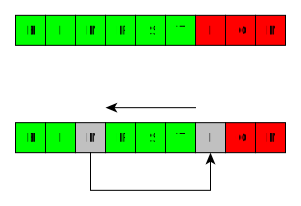
\includegraphics[scale=0.6]{figures/insertionsort_details.pdf}
    \end{center}
    \textbf{Exercice -} Quelle est la complexité au pire cas de cet algorithme ?
\end{frame}

\begin{frame}[fragile]{Tri par insertion}
    Fonctions de la librairie algorithmique :
    \begin{lstlisting}
template< class ForwardIt >
void rotate( ForwardIt first, ForwardIt n_first, ForwardIt last );

template< class ForwardIt, class T >
ForwardIt upper_bound( ForwardIt first, ForwardIt last, const T& value );
    \end{lstlisting}
    Illustation de \lstinline{std::rotate} dans \lstinline{rotate.cpp}.
\end{frame}


\begin{frame}[fragile]{Tri par insertion}
    \begin{lstlisting}
template <class ForwardIt>
void insertionsort(ForwardIt first, ForwardIt last)
{
    for (auto it = first; it != last; ++it) {
        std::rotate(std::upper_bound(first, it, *it), it, std::next(it));
    }
}
    \end{lstlisting}
\end{frame}

\begin{frame}[fragile]{Quicksort}
    \begin{lstlisting}
template <class ForwardIt>
void quicksort(ForwardIt first, ForwardIt last)
{
   if(first == last) return;
   auto pivot = *std::next(first, std::distance(first,last)/2);
   ForwardIt middle1 = std::partition(first, last, 
                        [pivot](const auto& em){ return em < pivot; });
   ForwardIt middle2 = std::partition(middle1, last, 
                        [pivot](const auto& em){ return !(pivot < em); });
   quicksort(first, middle1);
   quicksort(middle2, last);
}
    \end{lstlisting}
\end{frame}


\end{document}
